\documentclass[english,handout]{mlutalk}

\title{%
  Modern Talking: Key-Point Analysis \\
  using Modern Language Understanding
}
\subtitle{Natural Language Processing, Summer Semester 2021}
\author{Max Henze \and Hanh Luu \and Jan Heinrich Reimer}
\institute{Martin Luther University Halle-Wittenberg}
\date{June 29, 2021}
\titlegraphic{
\includegraphics[width=3cm]{figures/mlu-halle}}

\addbibresource{../literature/literature.bib}

\usepackage{tikz}
\usetikzlibrary{positioning}
\usepackage{listings}
\usepackage{xspace}
\usepackage{biblatex}
\usepackage{tabularx}
\usepackage{booktabs}
\usepackage{graphics,graphicx}

\newcommand{\ArgKP}{\mbox{ArgKP}\xspace}
\newcommand{\ArgQ}{\mbox{IBM-ArgQ-Rank-30kArgs}\xspace}
\newcommand{\BiLSTM}{\mbox{BiLSTM}\xspace}
\newcommand{\Bert}{\textsc{Bert}\xspace}
\newcommand{\BertBase}{\Bert-Base\xspace}
\newcommand{\BertLarge}{\Bert-Large\xspace}
\newcommand{\Roberta}{\mbox{Ro\textsc{Bert}a}\xspace}
\newcommand{\RobertaBase}{\Roberta-Base\xspace}
\newcommand{\TF}{\mbox{TF}\xspace}
\newcommand{\TFIDF}{\mbox{TF/IDF}\xspace}
\newcommand{\todocite}{{\smaller\color{red}[CITE]}\xspace}
\newcommand{\todo}[1]{{\smaller\color{red}[#1]}}

\tikzset{%
  every neuron/.style={
    circle,
    draw,
    minimum size=1cm,
  },
  layer/.style= {
    rectangle,
    draw,
    minimum size=1cm,
    rounded corners,
  }
}

\begin{document}

\titleframe

\begin{frame}[allowframebreaks]{Initial Ideas}
  
  \begin{itemize}
    \item Rule-based baseline 
      \begin{itemize}
        \item Lecture inspired us to try this approach
      \end{itemize}
    \item Improve upon the baseline with Machine Learning
    \begin{itemize}
      \item Regression, SVC~\cite{CortesV1995}
      \item Ensemble
      \item Deep Neural Networks, e.g., \BiLSTM~\cite{SchusterP1997,HochreiterS1997} with GloVe embeddings~\cite{PenningtonSM2014}, \Bert~\cite{DevlinCLT2018}
    \end{itemize}
    \item Variations of the above \(\to\) Hyper-parameter tuning
  \end{itemize}

  \framebreak
  
  \begin{block}{What did not work?}
    Some of the brainstormed ideas did not improve upon the baseline:
    \begin{itemize}
      \item Regression, SVC
      \item Ensemble
      \item \BiLSTM
      \begin{itemize}
        \item Integrating topic information in \BiLSTM resulted in better argument mining \cite{StabMSRG2018}
        \item Practical implementation proved to be challenging and resulted in no genuine improvements
      \end{itemize}
    \end{itemize}
  \end{block}
  
  \begin{block}{What did work?}
    \begin{itemize}
      \item \Bert
      \begin{itemize}
        \item State-of-the-art ML approach used widely in NLP problems with usually good performance
      \end{itemize}
    \end{itemize}
  \end{block}

\end{frame}



\begin{frame}[allowframebreaks]{Term Overlap}
  
  \begin{itemize}
    \item Rule-based approach with no training
    \item Features: (preprocessed) terms
    \item Preprocessing:
    \begin{itemize}
      \item Stemming \(\leadsto\) generalization
      \item Stop words \(\leadsto\) less noise/confusion \\ modified without \query{not}
      \item Synonyms, antonyms \(\leadsto\) generalization
    \end{itemize}
    \item Compute similarity based on Jaccard similarity coefficient~\cite{Jaccard1902}, \\ i.e., proportion of terms that appear in argument and key point
    \item Good improvement with preprocessing: up to 12~pp 
  \end{itemize}
  
  \begin{example}[Preprocessing]
    \smaller
    Homeschooling a child denies them valuable lifeskills, particularly interaction with their own age group and all experiences stemming from this. \\
    \(\to\) homeschool child deni valuabl lifeskil particular interact age group experi stem
  \end{example}

  \framebreak
  
  \begin{block}{Technology}
      \begin{itemize}
        \item NLTK~\cite{Bird2006} for tokenization, stemming,  and stop word list
        \item WordNet~\cite{Miller1995} (via NLTK) for synonyms and antonyms
      \end{itemize}
  \end{block}

  \begin{block}{Intuition}
    \begin{itemize}
      \item Many arguments contain the same words as matching key points
      \item Key points summarize arguments
      \item Stemming/synonyms/antonyms increase overlap
    \end{itemize}

    \begin{example}
      \smaller
      \begin{tabular}{lp{0.7\textwidth}}
        Argument: & People reach their limit when it comes to their quality of life and should be able to end their {\color{blue} suffering}. This can be done with little or no {\color{blue} suffering} by {\color{orange} assistance} and the person is able to say good bye. \\
        Key Point: & {\color{orange} Assisted} suicide reduces {\color{blue} suffering}.
      \end{tabular}
    \end{example}
  \end{block}

\end{frame}

\begin{frame}{Regression, SVC}
  
  \framesubtitle{What did not work?}
  
  \begin{itemize}
    \item Features: bag-of-words and/or \TFIDF for selected parts-of-speech
    \item Logistic regression, Support Vector Classifier
    \item Ensemble of Regression + SVC
  \end{itemize}
  
  \begin{block}{Technology}
      \begin{itemize}
        \item NLTK~\cite{Bird2006} for stemming
        \item spaCy~\cite{HonnibalMVLB2020} for part-of-speech tagging
        \item Scikit-Learn~\cite{PedregosaVGMTGBPWDVPCBPD2011} for bag-of-words and \TFIDF
        \item Scikit-Learn~\cite{PedregosaVGMTGBPWDVPCBPD2011} for regression and SVC implementation
      \end{itemize}
  \end{block}

\end{frame}

\begin{frame}{Regression, SVC}

  \framesubtitle{Why did it not work?}

  \begin{itemize}
    \item Too much features~(\( > 4000 \)) for Regression
    \item SVC better results, but still worse than baseline
    \item Can't capture context or semantic meaning
  \end{itemize}

  \begin{example}[False Positives]
    \smaller
    \begin{tabular}{ll}
      Argument: & School uniforms violate the right to freedom of expression. \\
      Key Point: & School uniforms are often uncomfortable/sexist. \\
      Prediction: & Match
    \end{tabular}
  \end{example}
  
  \begin{example}[False Negatives]
    \smaller
    \begin{tabular}{ll}
      Argument: & It is not fair to not allow children to express their personality through dress as long as it is appropriate. \\
      Key Point: & School uniform is harming the student's self expression. \\
      Prediction: & No match
    \end{tabular}
  \end{example}

\end{frame}

\begin{frame}[allowframebreaks]{Bidirectional LSTM}
  
  \framesubtitle{What did not work?}
  
  \begin{itemize}
    \item Embed with GloVe~\cite{PenningtonSM2014}
    \item Encode argument and key point separately \\ with bidirectional long short-term memory~(\BiLSTM) model~\todocite
    \item Encode merged sequences with \BiLSTM
    \item Classify pooled output to estimate similarity
  \end{itemize}
  
  \begin{block}{Preprocessing}
      \begin{itemize}
        \item Missing labels in training data
        \begin{description}
          \item[skip] Use only labeled pairs
          \item[strict] Assume no match
          \item[relaxed] Assume match
        \end{description}
        \item Data augmentation with WordNet~\cite{Miller1995} synonyms and misspellings
      \end{itemize}
  \end{block}

  \framebreak

  \begin{figure}
    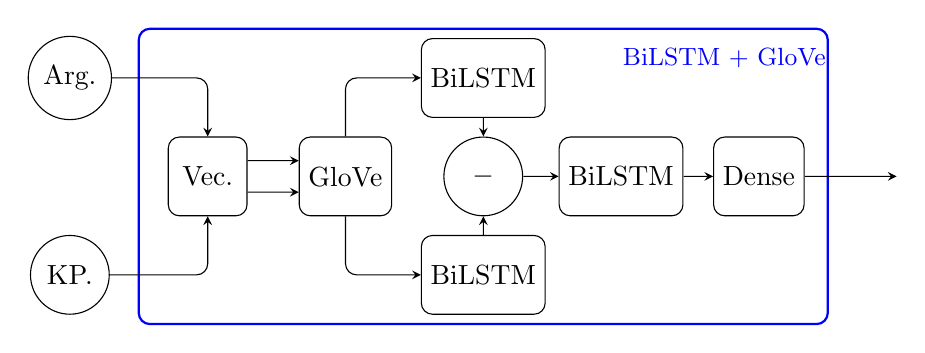
\begin{tikzpicture}[xscale=1.75, yscale=2.5, >=stealth]
      \node[every neuron] (arg) at (0, 1) {Arg.};
      \node[every neuron] (kp) at (0, 0) {KP.};
      \node[layer] (vec) at (1, 0.5) {Vec.};
      \node[layer] (glove) at (2, 0.5) {GloVe};
      \node[layer] (bilstm-arg) at (3, 1) {\BiLSTM};
      \node[layer] (bilstm-kp) at (3, 0) {\BiLSTM};
      \node[every neuron] (merge) at (3, 0.5) {\(-\)};
      \node[layer] (bilstm) at (4, 0.5) {\BiLSTM};
      \node[layer] (dense) at (5, 0.5) {Dense};
      \node at (4.75, 1.1) {\small\color{blue} \BiLSTM + GloVe};
      \draw[draw=blue, rounded corners, thick] (0.5, -0.25) rectangle (5.5, 1.25);
      \draw[->, rounded corners] (arg) -| (vec);
      \draw[->, rounded corners] (kp) -| (vec);
      \draw[->, transform canvas={yshift=-2mm}] (vec) -- (glove);
      \draw[->, transform canvas={yshift=2mm}] (vec) -- (glove);
      \draw[->, rounded corners] (glove) |- (bilstm-arg);
      \draw[->, rounded corners] (glove) |- (bilstm-kp);
      \draw[->] (bilstm-arg) -- (merge);
      \draw[->] (bilstm-kp) -- (merge);
      \draw[->] (merge) -- (bilstm);
      \draw[->] (bilstm) -- (dense);
      \draw[->] (dense) -- (6, 0.5);
    \end{tikzpicture}
    \caption{\BiLSTM + GloVe model}
  \end{figure}
  
  \begin{block}{Technology}
      \begin{itemize}
        \item TensorFlow~\cite{Abadi2015} and Keras~\cite{Chollet2015} for model layers~(e.g., RNN) and tokenization
        \item NLPAug~\cite{Edward2019} for data augmentation
      \end{itemize}
  \end{block}

\end{frame}

\begin{frame}{Bidirectional LSTM}
  \framesubtitle{Why doesn't it work?}

  \begin{itemize}
    \item Complex hyper-parameters
    \item Epochs
    \begin{itemize}
      \item Too few~(1--10) \(\to\) okay on training set but no generalization on dev set
      \item Too much~(10--100) \(\to\) overfiting
    \end{itemize}
    \item Slow learning rate~\(\eta = 0.0001\) does not improve much
    \item Early stopping, dropout layers, and weight decay \(\to\) neglible improvements
    \item Generate new samples~(data augmentation) \(\to\) \textquote{confuses} model
  \end{itemize}

  \begin{block}{Conclusion}
    \BiLSTM model probably to difficult or wrong way of data input.
  \end{block}

\end{frame}

\begin{frame}{\Bert and Transformers}

  \begin{itemize}
    \item Pretrained encoder model, e.g., \Bert~\cite{DevlinCLT2018} or \Roberta~\todocite
    \item Sequence classification model \\ \(=\) dense layer after \Bert pooling output
    \item Input: pairs of argument and key point texts
    \item Fine-tune pretrained model with ArgKP data
  \end{itemize}
  
  \begin{block}{Parameters}
    \begin{itemize}
    		\item Missing labels: skip, relaxed, strict (like for \BiLSTM)
    		\item Data augmentation
    		\item Batch size, epochs, learning rate, \ldots
    \end{itemize}
  \end{block}
  
  \begin{block}{Technology}
    \begin{itemize}
      \item Simple Transformers~\cite{Rajapaske2019} for tokenization, model, and training
      \item NLPAug~\cite{Edward2019} for data augmentation
    \end{itemize}
  \end{block}

\end{frame}

\begin{frame}{\Roberta~\todocite}

  Alternative language model (pretrained encoder).

  \begin{block}{Better than \Bert?\footnote{\tiny\smaller\url{https://towardsdatascience.com/bert-roberta-distilbert-xlnet-which-one-to-use-3d5ab82ba5f8}}}
    \begin{itemize}
      \item Trained on 160~GB of data vs 16~GB (\Bert)
      \item Larger mini-batches, learning rates, and step sizes \(\to\) longer training
      \item Often 2--20\,\% improvement over \Bert
    \end{itemize}
  \end{block}

  \begin{block}{Hyper-parameter settings}
    \begin{itemize}
      \item 
    \end{itemize}
  \end{block}
\end{frame}

\begin{frame}{Evaluation}
  \framesubtitle{Mean Average Precision}
  \begin{figure}
    \centering
    \caption{Mean average precision of the match label for different approaches and baselines, as computed by the KPA\,2021 Shared Task's evaluation script.
    Values where the script returns no score are indicated by ---.}
    \tiny
    \begin{tabular}{lcccccc}
      \toprule
      \textbf{Baselines/Approach} & \multicolumn{3}{c}{\textbf{Training Data}} & \multicolumn{3}{c}{\textbf{Validation Data}}\\
      \cmidrule(r{0.5em}){2-4} \cmidrule(l{0.5em}){5-7}
      & Strict & Relaxed & Average & Strict & Relaxed & Average\\
      \midrule
      Random 
      & ---   & ---   & ---   & 0.188 & 0.365 & 0.277 \\
      Term Overlap (no preprocessing)
      & 00000 & 00000 & 00000 & 00000 & 00000 & 00000 \\
      Term Overlap (with preprocessing)
      & 00000 & 00000 & 00000 & 00000 & 00000 & 00000 \\
      \midrule
      BiLSTM (GloVe embeddings)
      & 00000 & 00000 & 00000 & 00000 & 00000 & 00000 \\
      \BertBase
      & 00000 & 00000 & 00000 & 00000 & 00000 & 00000 \\
      \RobertaBase
      & 00000 & 00000 & 00000 & 00000 & 00000 & 00000 \\
      \bottomrule
    \end{tabular}
  \end{figure}
\end{frame}

\begin{frame}{Evaluation}
  \framesubtitle{Mean Average Precision (fixed)}
  \begin{figure}
    \centering
    \caption{Mean average precision of the match label for different approaches and baselines, as described in the KPA\,2021 Shared Task's documentation.}
    \tiny
    \begin{tabular}{lcccccc}
      \toprule
      \textbf{Baselines/Approach} & \multicolumn{3}{c}{\textbf{Training Data}} & \multicolumn{3}{c}{\textbf{Validation Data}}\\
      \cmidrule(r{0.5em}){2-4} \cmidrule(l{0.5em}){5-7}
      & Strict & Relaxed & Average & Strict & Relaxed & Average\\
      \midrule
      Random 
      & 0.170 & 0.307 & 0.238 & 0.188 & 0.365 & 0.277 \\
      Term Overlap (no preprocessing)
      & 00000 & 00000 & 00000 & 00000 & 00000 & 00000 \\
      Term Overlap (with preprocessing)
      & 00000 & 00000 & 00000 & 00000 & 00000 & 00000 \\
      \midrule
      BiLSTM (GloVe embeddings)
      & 00000 & 00000 & 00000 & 00000 & 00000 & 00000 \\
      \BertBase
      & 00000 & 00000 & 00000 & 00000 & 00000 & 00000 \\
      \RobertaBase
      & 00000 & 00000 & 00000 & 00000 & 00000 & 00000 \\
      \bottomrule
    \end{tabular}
  \end{figure}
\end{frame}

\begin{frame}{Evaluation}
  \framesubtitle{Precision}
  \begin{figure}
    \centering
    \caption{Precision of the match label for different approaches and baselines.}
    \tiny
    \begin{tabular}{lcccccc}
      \toprule
      \textbf{Baselines/Approach} & \multicolumn{3}{c}{\textbf{Training Data}} & \multicolumn{3}{c}{\textbf{Validation Data}}\\
      \cmidrule(r{0.5em}){2-4} \cmidrule(l{0.5em}){5-7}
      & Strict & Relaxed & Average & Strict & Relaxed & Average\\
      \midrule
      Random 
      & 0.176 & 0.330 & 0.253 & 0.179 & 0.344 & 0.261 \\
      Term Overlap (no preprocessing)
      & 00000 & 00000 & 00000 & 00000 & 00000 & 00000 \\
      Term Overlap (with preprocessing)
      & 00000 & 00000 & 00000 & 00000 & 00000 & 00000 \\
      \midrule
      BiLSTM (GloVe embeddings)
      & 00000 & 00000 & 00000 & 00000 & 00000 & 00000 \\
      \BertBase
      & 00000 & 00000 & 00000 & 00000 & 00000 & 00000 \\
      \RobertaBase
      & 00000 & 00000 & 00000 & 00000 & 00000 & 00000 \\
      \bottomrule
    \end{tabular}
  \end{figure}
\end{frame}

\begin{frame}{Evaluation}
  \framesubtitle{Macro Precision}
  \begin{figure}
    \centering
    \caption{Macro precision of both labels for different approaches and baselines.}
    \tiny
    \begin{tabular}{lcccccc}
      \toprule
      \textbf{Baselines/Approach} & \multicolumn{3}{c}{\textbf{Training Data}} & \multicolumn{3}{c}{\textbf{Validation Data}}\\
      \cmidrule(r{0.5em}){2-4} \cmidrule(l{0.5em}){5-7}
      & Strict & Relaxed & Average & Strict & Relaxed & Average\\
      \midrule
      Random 
      & 0.334 & 0.333 & 0.334 & 0.336 & 0.326 & 0.331 \\
      Term Overlap (no preprocessing)
      & 00000 & 00000 & 00000 & 00000 & 00000 & 00000 \\
      Term Overlap (with preprocessing)
      & 00000 & 00000 & 00000 & 00000 & 00000 & 00000 \\
      \midrule
      BiLSTM (GloVe embeddings)
      & 00000 & 00000 & 00000 & 00000 & 00000 & 00000 \\
      \BertBase
      & 00000 & 00000 & 00000 & 00000 & 00000 & 00000 \\
      \RobertaBase
      & 00000 & 00000 & 00000 & 00000 & 00000 & 00000 \\
      \bottomrule
    \end{tabular}
  \end{figure}
\end{frame}

\begin{frame}{Evaluation}
  \framesubtitle{Recall}
  \begin{figure}
    \centering
    \caption{Recall of the match label for different approaches and baselines.}
    \tiny
    \begin{tabular}{lcccccc}
      \toprule
      \textbf{Baselines/Approach} & \multicolumn{3}{c}{\textbf{Training Data}} & \multicolumn{3}{c}{\textbf{Validation Data}}\\
      \cmidrule(r{0.5em}){2-4} \cmidrule(l{0.5em}){5-7}
      & Strict & Relaxed & Average & Strict & Relaxed & Average\\
      \midrule
      Random 
      & 0.504 & 0.499 & 0.501 & 0.522 & 0.496 & 0.509 \\
      Term Overlap (no preprocessing)
      & 00000 & 00000 & 00000 & 00000 & 00000 & 00000 \\
      Term Overlap (with preprocessing)
      & 00000 & 00000 & 00000 & 00000 & 00000 & 00000 \\
      \midrule
      BiLSTM (GloVe embeddings)
      & 00000 & 00000 & 00000 & 00000 & 00000 & 00000 \\
      \BertBase
      & 00000 & 00000 & 00000 & 00000 & 00000 & 00000 \\
      \RobertaBase
      & 00000 & 00000 & 00000 & 00000 & 00000 & 00000 \\
      \bottomrule
    \end{tabular}
  \end{figure}
\end{frame}

\begin{frame}{Evaluation}
  \framesubtitle{Macro Recall}
  \begin{figure}
    \centering
    \caption{Macro recall of both labels for different approaches and baselines.}
    \tiny
    \begin{tabular}{lcccccc}
      \toprule
      \textbf{Baselines/Approach} & \multicolumn{3}{c}{\textbf{Training Data}} & \multicolumn{3}{c}{\textbf{Validation Data}}\\
      \cmidrule(r{0.5em}){2-4} \cmidrule(l{0.5em}){5-7}
      & Strict & Relaxed & Average & Strict & Relaxed & Average\\
      \midrule
      Random 
      & 0.335 & 0.333 & 0.334 & 0.338 & 0.326 & 0.332 \\
      Term Overlap (no preprocessing)
      & 00000 & 00000 & 00000 & 00000 & 00000 & 00000 \\
      Term Overlap (with preprocessing)
      & 00000 & 00000 & 00000 & 00000 & 00000 & 00000 \\
      \midrule
      BiLSTM (GloVe embeddings)
      & 00000 & 00000 & 00000 & 00000 & 00000 & 00000 \\
      \BertBase
      & 00000 & 00000 & 00000 & 00000 & 00000 & 00000 \\
      \RobertaBase
      & 00000 & 00000 & 00000 & 00000 & 00000 & 00000 \\
      \bottomrule
    \end{tabular}
  \end{figure}
\end{frame}

\begin{frame}{Evaluation}
  \framesubtitle{F1-Score}
  \begin{figure}
    \centering
    \caption{F1-Score of the match label for different approaches and baselines.}
    \tiny
    \begin{tabular}{lcccccc}
      \toprule
      \textbf{Baselines/Approach} & \multicolumn{3}{c}{\textbf{Training Data}} & \multicolumn{3}{c}{\textbf{Validation Data}}\\
      \cmidrule(r{0.5em}){2-4} \cmidrule(l{0.5em}){5-7}
      & Strict & Relaxed & Average & Strict & Relaxed & Average\\
      \midrule
      Random 
      & 0.261 & 0.397 & 0.329 & 0.267 & 0.406 & 0.336 \\
      Term Overlap (no preprocessing)
      & 00000 & 00000 & 00000 & 00000 & 00000 & 00000 \\
      Term Overlap (with preprocessing)
      & 00000 & 00000 & 00000 & 00000 & 00000 & 00000 \\
      \midrule
      BiLSTM (GloVe embeddings)
      & 00000 & 00000 & 00000 & 00000 & 00000 & 00000 \\
      \BertBase
      & 00000 & 00000 & 00000 & 00000 & 00000 & 00000 \\
      \RobertaBase
      & 00000 & 00000 & 00000 & 00000 & 00000 & 00000 \\
      \bottomrule
    \end{tabular}
  \end{figure}
\end{frame}

\begin{frame}{Evaluation}
  \framesubtitle{Macro F1-Score}
  \begin{figure}
    \centering
    \caption{Macro F1-score of both labels for different approaches and baselines.}
    \tiny
    \begin{tabular}{lcccccc}
      \toprule
      \textbf{Baselines/Approach} & \multicolumn{3}{c}{\textbf{Training Data}} & \multicolumn{3}{c}{\textbf{Validation Data}}\\
      \cmidrule(r{0.5em}){2-4} \cmidrule(l{0.5em}){5-7}
      & Strict & Relaxed & Average & Strict & Relaxed & Average\\
      \midrule
      Random 
      & 0.295 & 0.323 & 0.309 & 0.295 & 0.318 & 0.306 \\
      Term Overlap (no preprocessing)
      & 00000 & 00000 & 00000 & 00000 & 00000 & 00000 \\
      Term Overlap (with preprocessing)
      & 00000 & 00000 & 00000 & 00000 & 00000 & 00000 \\
      \midrule
      BiLSTM (GloVe embeddings)
      & 00000 & 00000 & 00000 & 00000 & 00000 & 00000 \\
      \BertBase
      & 00000 & 00000 & 00000 & 00000 & 00000 & 00000 \\
      \RobertaBase
      & 00000 & 00000 & 00000 & 00000 & 00000 & 00000 \\
      \bottomrule
    \end{tabular}
  \end{figure}
\end{frame}

\begin{frame}{Conclusion}
  \begin{itemize}
    \item Strong, rule-based baseline
    \item Creative model ideaa, though not better than baseline
    \item \Roberta better able to capture semantic similarity
    \item Submitted scores (on validation data): \\
    \begin{tabular}{@{}lc}
      mAP strict: & 00000 \\
      mAP relaxed: & 00000
    \end{tabular}
  \end{itemize}
\end{frame}

\appendix
\section{\appendixname}

\bibliographyframe

\end{document}